\section{XACML Policy Refactoring Process} \label{sec:approach}
This section describes our approach of refactoring access control policies to improve performance by reducing the number of policy rules. 
For refactoring policies in a systematic way, we propose seven policy splitting criteria
based on attribute set. Moreover, we explain how to select the splitting criterion, which preserves the synergy requirement in the access control architecture. 

 


\subsection{Definition of Policy based Splitting Criteria}


Given a request, a PDP adopts brute force searching to find its decision
by evaluating the request against policy rules one by one until the PDP finds an evaluation decision.
For request evaluation processing, not of all the rules are applicable to the request.
In order words, only part of the rules (i.e., relevant rules) are applicable to the request and can contribute
to determine a final authorization decision.
We propose an approach to evaluate a request against only the relevant rules for a given request by refactoring
access control policies.
  
%Our approach is to split a single global policy into multiple policies based on attributes combination. 
Our approach refactors a policy into a set of sub-policies where the rules have the same values of attributes of subject, resource, or 
action.
Formally, our approach refactors an policy \normalsize $P$ into 
multiple policies \normalsize $P_{SC_{w}}$ based on Splitting Criteria $SC_{w}$.
These multiple policies contain less number of rules (compared to the number of rules in \normalsize $P$) and conforms to a Splitting Criteria $SC_{w}$. An $SC_{w}$ defines the set of attributes, which classify all of policy rules into subsets with the same attribute values for
selected attributes.
$w$ denotes the number of attributes that have to be considered conjointly for aggregating 
rules based on selected attributes. 


 
We first consider two attributes (e.g., $\langle Subject, Action\rangle$ or $\langle Action$, $Resource\rangle$) for Splitting Criteria. In such a setting, our approach refactors a policy into a set of 
policies each of which rules include the same couple of attribute elements. For example, $\langle Subject, Action\rangle$ criterion
classifies rules with same subjects and actions into sub-policies.
We also extend our Splitting Criteria by considering three attributes such as resource, action, and subject.
Table~\ref{table1} shows our proposed splitting criteria categories according to the attribute elements combination.

\begin{table}[h!]
\centering
\setlength{\extrarowheight}{6 pt}
\begin{tabular}{|>{\small}c|>{\small}c|} 
\hline  \rowcolor{black} 
\bf
\textcolor{white}{Categories}& \bf \textcolor{white}{Splitting Criteria}\\ \hline
$SC_{1}$& {$\langle Subject \rangle, \langle Resource\rangle, \langle Action\rangle$}\\ \hline
$SC_{2}$& {$\langle Subject,Action \rangle, \langle Subject,Resource\rangle$}\\&{$\langle Resource,Action\rangle$}\\  \hline
$SC_{3}$& {$\langle Subject,Resource,Action\rangle$}\\ \hline
\end{tabular}
\caption{Splitting Criteria}
\label{table1}\end{table}



Once the splitting process is performed, the access control architecture will include one or more (PDPs) that comply with a certain splitting criterion.
We use SUN PDP \cite{sunxacml} as a decision engine framework that evaluates requests against the policies specified in XACML.
During the evaluation process, SUN PDP checks the request against the policy and determines whether its authorization
decision is 
permit or deny. SUN PDP permits to load the considered policy in a file which is used during the decision making process, once the applicable policy 
is selected from this file, the decision engine fetches the policy to retrieve the applicable rules that are applicable to the request.


Figure \ref{requestevaluation} presents an evaluation process that considers resulting policies from the splitting process. 
During the evaluation process the applicable 
policy is selected from the configuration file. Sun's XACML enables to select the applicable policy, by verifying the matching between the request's attributes
 and the policy set attributes. 
After the selection of the applicable policy, all its rules which are considered relevant for the decision making are evaluated.

\begin{figure}[!h]
\begin{center}
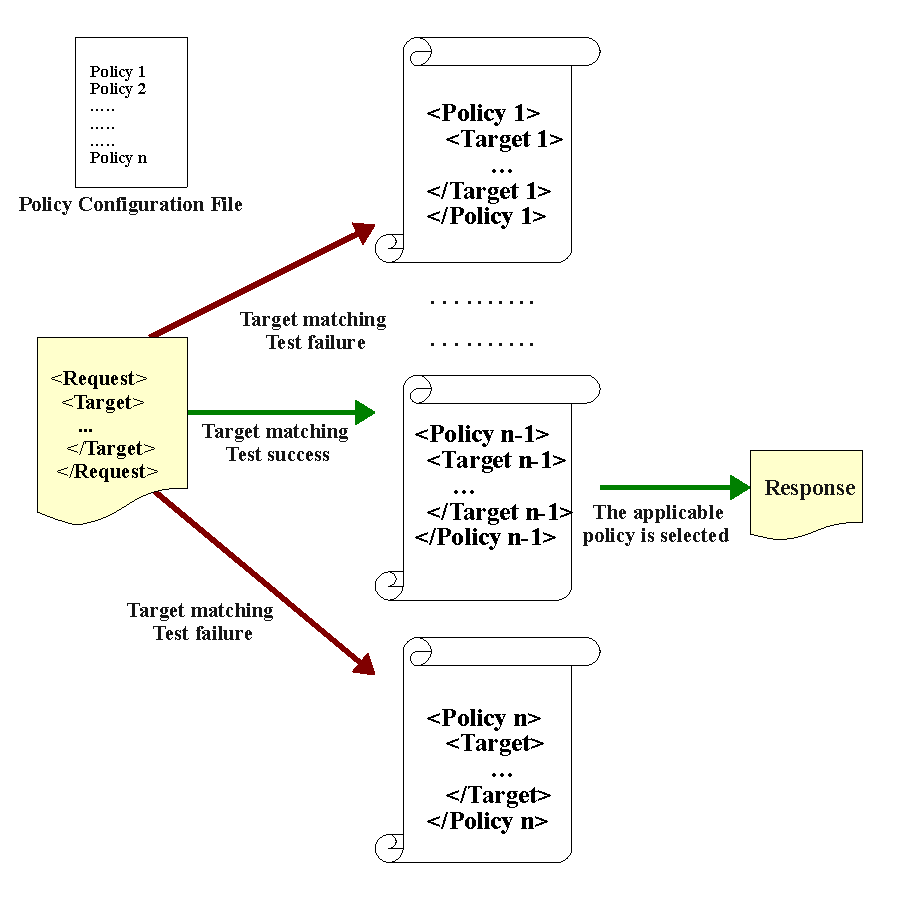
\includegraphics[width=3in, height=3in]{requestevaluation}
\caption{Applicable policy Selection}
\label{requestevaluation}
\end{center}
\end{figure}

As depicted in Figure \ref{overallprocess}, the refactoring process is automated and starts by specifying and creating the XACML file which 
will be split by our tool according to a specified SC that can be chosen by an access control stakeholder. Afterwards, the policies are included in the 
framework that supports our approach. For every change in the access control policy, the initial policy is updated and 
split again in order to be included again in the framework.
From a point of view of the system administration, maintaining and updating the access control policies is completely a standalone and simple
 process. The input is usually a centralized XACML policy. This input remains the same than before the access control performance issue is tackled.
Our process is transparent in the sense that it does not impact the existing functional aspects of the access control management system, 
for system administrators, who have to update the policy frequently and have to manage various dimensions of access control 
systems such the scalability and maintainability.
\begin{figure}[!h]
\begin{center}
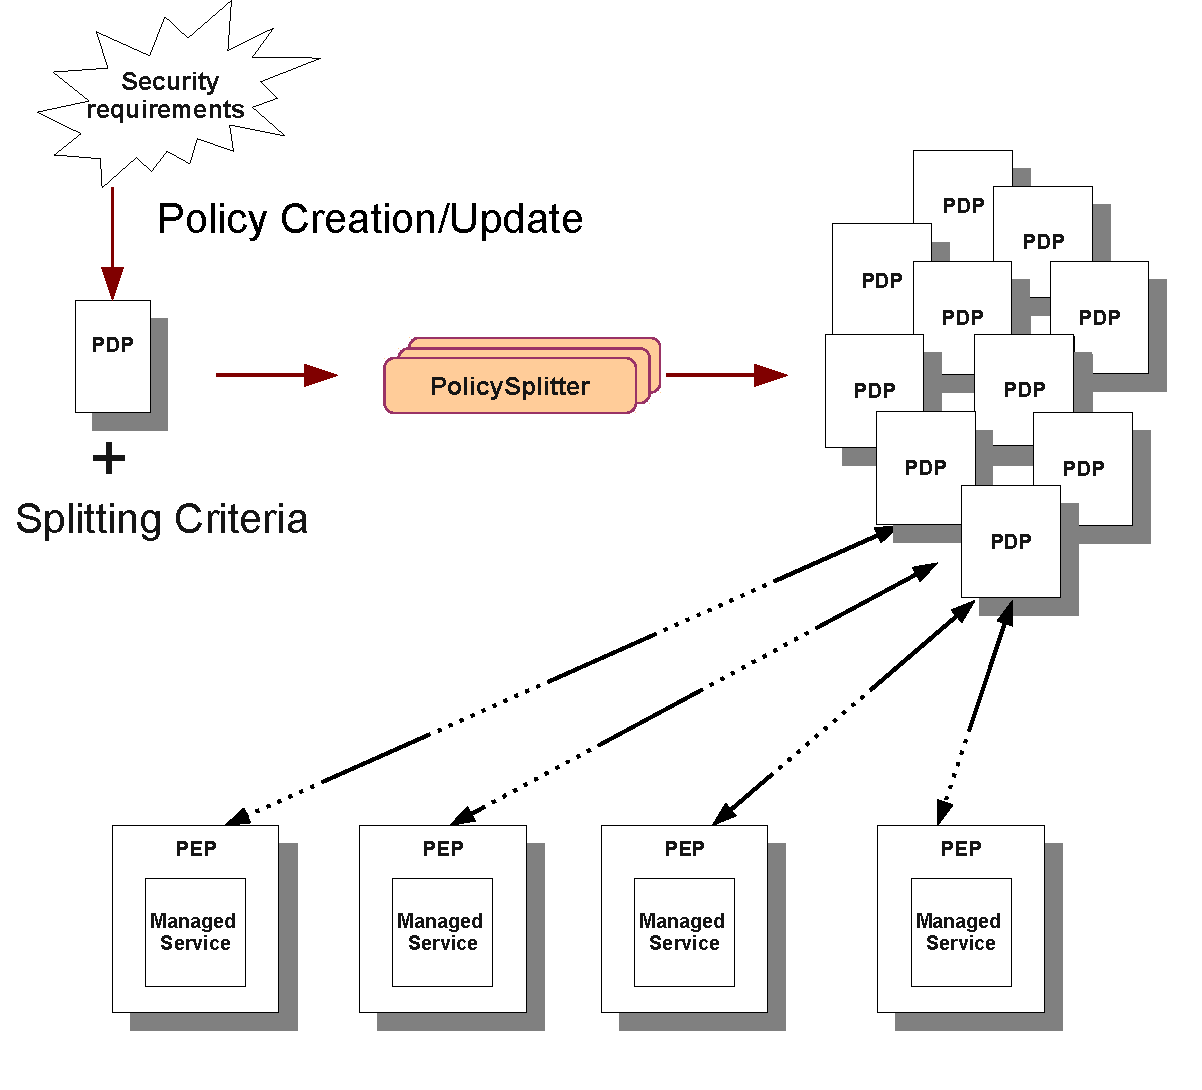
\includegraphics[width=8.5cm, height=8cm]{Overall-process}
\caption{Overview of the Refactoring Process}
\label{overallprocess}
\end{center}
\end{figure} 

To illustrate our approach, we present some examples that take into consideration the XACML language features:
\begin{itemize}
\item The refactoring of the XACML policy $P$ presented in Figure \ref{splitting} according to the splitting criterion $SC_{1}=\langle Subject\rangle$ consists in splitting $P$ 
into sub-policies $Pa$ and $Pb$ where each sub-policy groups the rules that are relevant to the same subject (Alice and Bob in this case). 

\item
XACML target elements may have an intricate structure, if they encapsulate the following elements $\langle Resou\-rceMatch\rangle$, $\langle SubjectMatch\rangle$, $\langle ActionMatch\rangle$.
These elements define a set of target elements related entities that match at the decision level with the context element in 
an access control request. In the example, shown in Figure\ref{xacml-match}, subject attribute includes two attributes (one is "role" and the other is "isEq-subjUserId-resUserId"). 
This subject can match with a request if the request has that at least role is pc-member and isEq-subjUserId-resUserId is true. In such configuration, the whole element subject is considered 
as a single entity that is not splitted by our supporting tool.

\item 

In XACML, policies and requests could be multi-valued. For example, the subject in a given request could both be the manager and the employee as a principal.
For the sake of simplicity, we don't consider multi-valued requests in this work.
\end{itemize}
\begin{figure}[!h]
\begin{center}
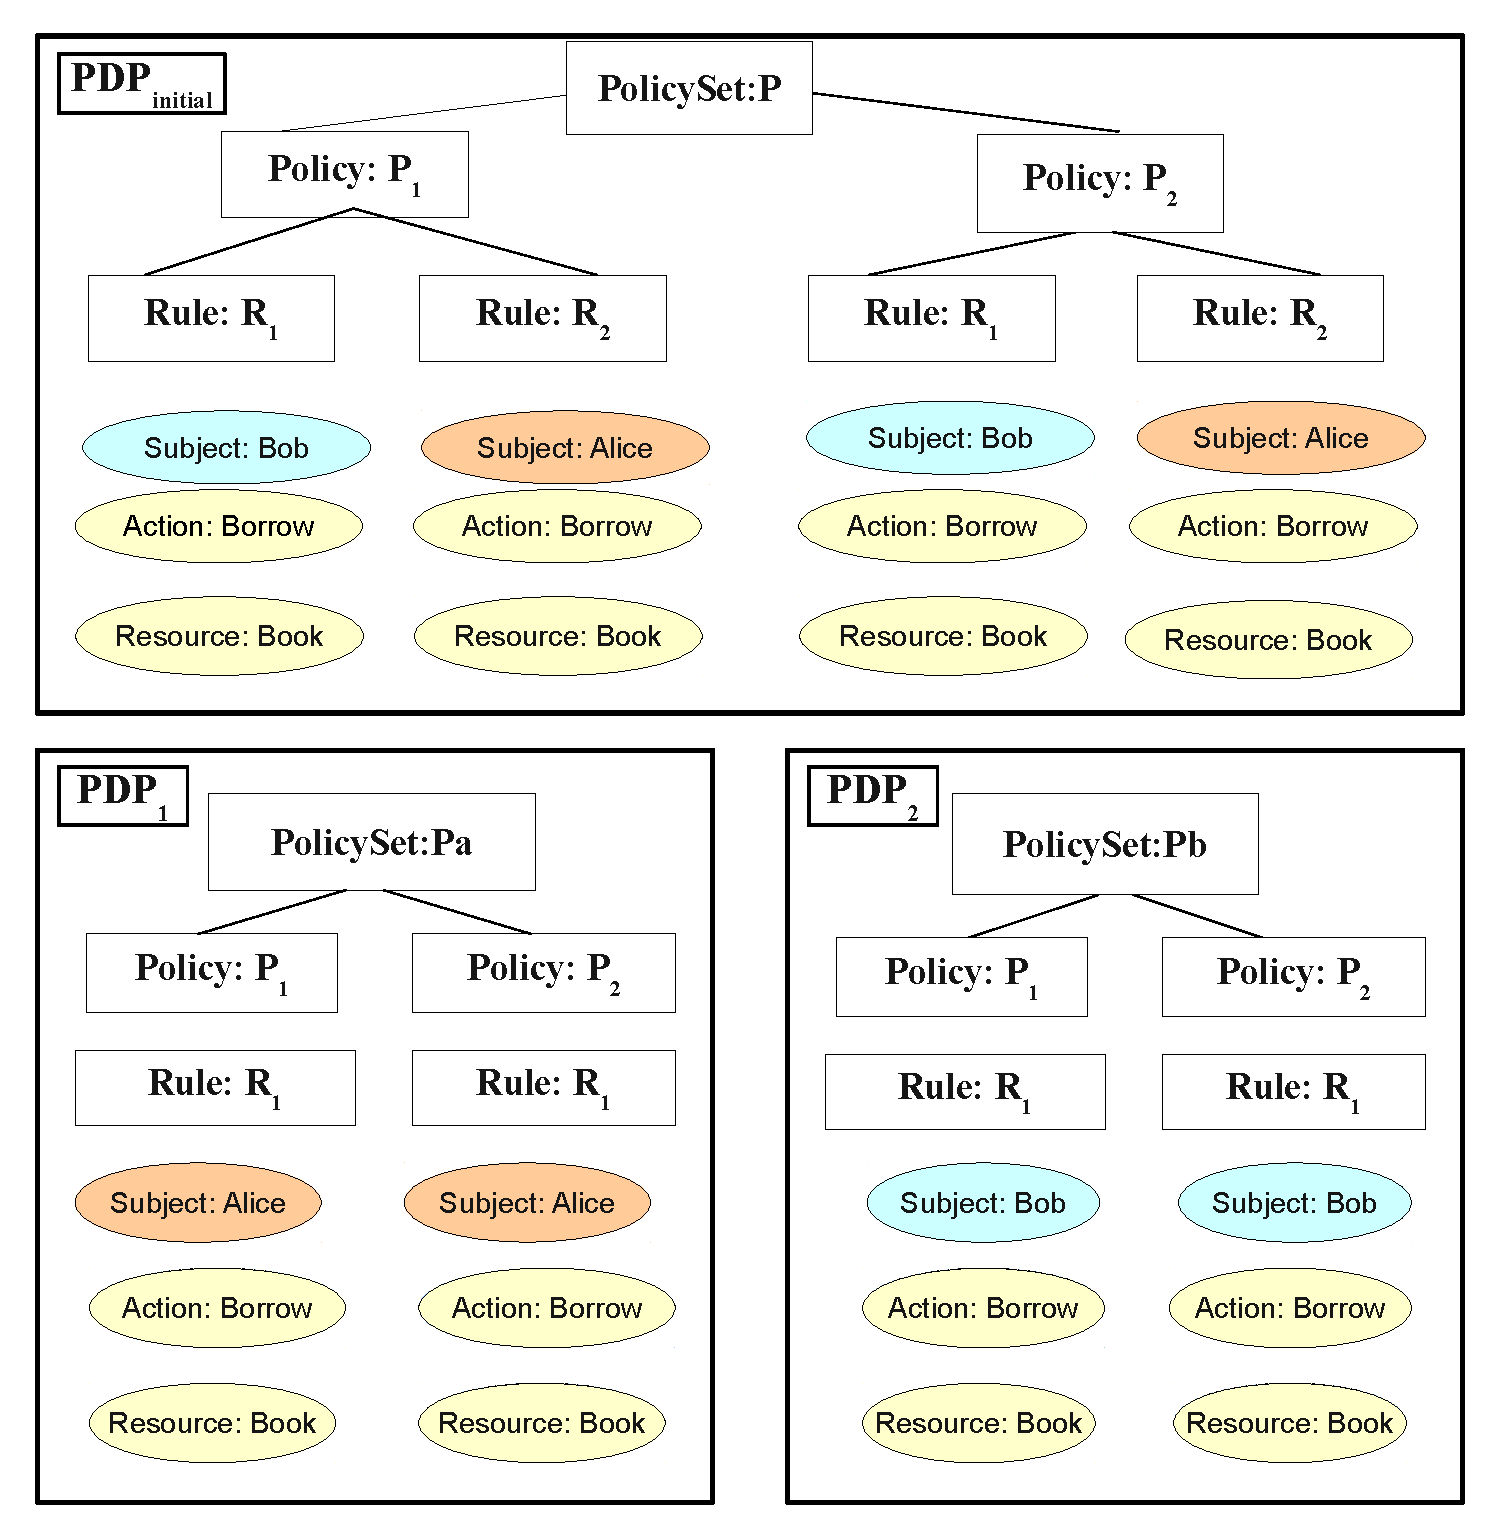
\includegraphics[width=8.5cm, height=7cm]{splitting}
\caption{Splitting a Policy according to $SC_{1}=\langle Subject\rangle$}
\label{splitting}
\end{center}
\end{figure} 


\begin{figure}[!h]
\begin{center}
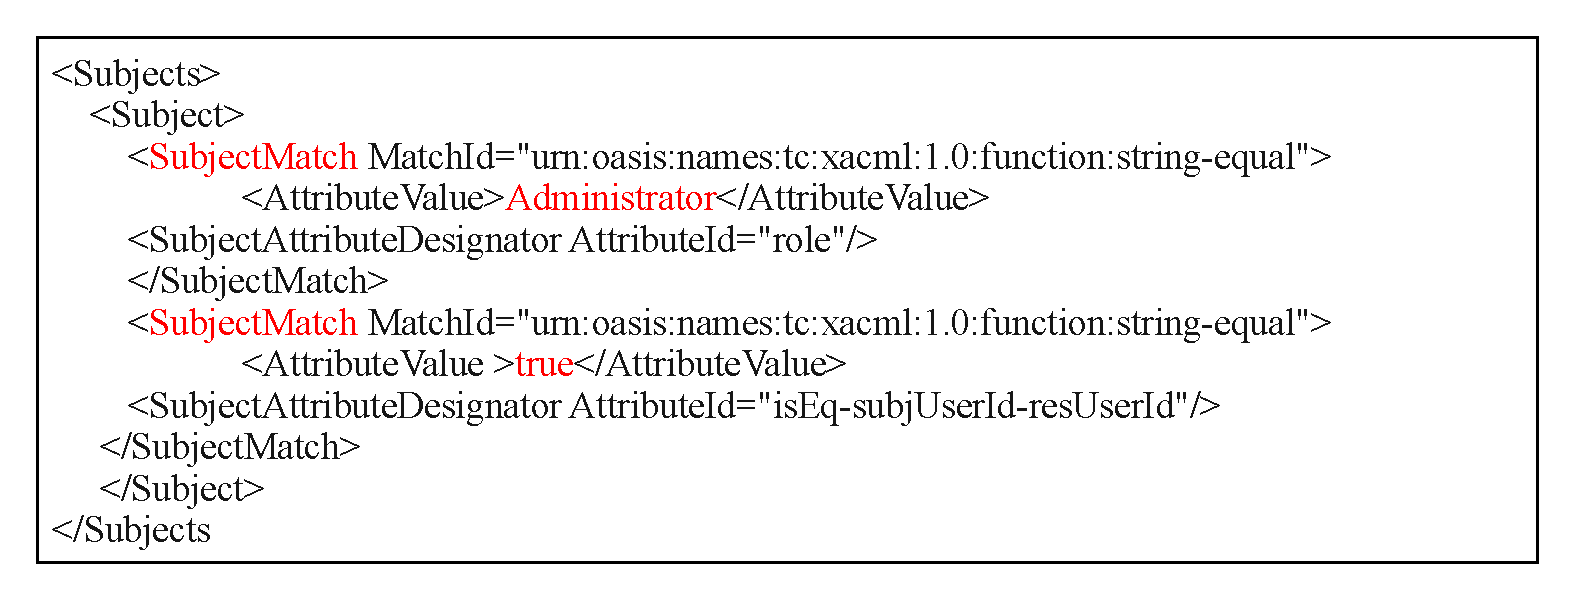
\includegraphics[width=9cm, height=3.5cm]{xacml-match}
\caption{Multi-attributes values Target Element}
\label{xacml-match}
\end{center}
\end{figure}
 


\subsection{Architecture Model Preservation: PEP-PDP Synergy}
We consider the different splitting criteria that we have identified in the previous section and we propose to select the splitting criterion that 
enables to preserve the synergy requirement in the access control architecture, this splitting criterion enables to have a valid refactoring and respects how PEPs are organized 
at the application level and how they are linked to their corresponding PDPs.

In the worst case, splitting the initial PDP into multi-PDPs may lead to a non-synergic system: a PEP may send its requests to several PDPs. 
The PDP, which receives a request is only known at runtime. Such a resulting architecture breaks the PEP-PDP synergy and the conceptual 
simplicity of the initial architecture model. In the best case, the refactoring preserves the simplicity of the initial architecture, by keeping a many-to-one association 
from PEPs to PDPs. A given request evaluation triggered by one PEP will always be handled by the same PDP. Operationally, the request evaluation process will involve 
one XACML policy file. In this case, the refactoring is valid, since its does not impact the conceptual architecture of the system.

A deep analysis of the PEPs at the application enables to observe the mapping between the PEPs and the PDP. At the application level, the PEP
is represented by a method call that triggers a decision making process by activating some specific rules in the PDP.
The code in Figure \ref{PEP deployment Example} is taken from \cite{legacy}, this code excerpt shows an example of a PEP represented by the method checkSecurity which calls the class 
SecurityPolicyService that initiates the PDP component.
\begin{figure}[!h]
\begin{center}
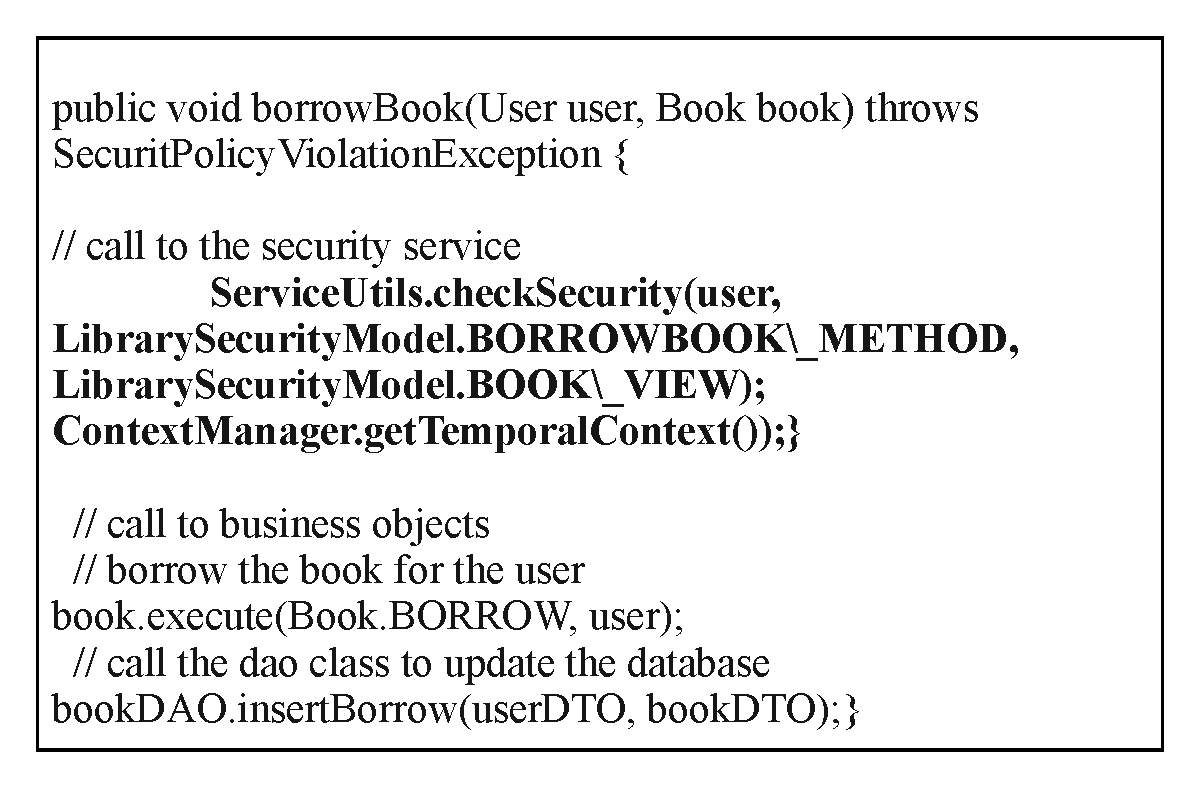
\includegraphics[width=7.5cm, height=4cm]{PEPExample}
\caption{PEP deployment Example}
\label{PEP deployment Example}
\end{center}
\end{figure}

An analysis of this code reflects that the PEP presented by the method ServiceUtils.checkSecurity will trigger exclusively all the rules 
that have the subject user (provided as input parameter in the PEP) and fixed Action and Resource (LibrarySecurityModel.BORROWBOOK\_METHOD), ( LibrarySecurityModel.BOOK\_VIEW).
Thus the splitting process that will preserve the mapping between the PEPs and the PDP is $SC_{2}=\langle Resource,Action\rangle$ since the rules in the policy are triggered 
by Action, Resource. Depending on the organization of the PEPs in a given application, connecting the rules with their PEPs at the application level may require to identify
 all the enforcements points in the application, and to track the different method calls triggered from these specific enforcement calls to map them to the relevant access control rules.

Our empirical results, presented in section~\ref{sec:experiment}, have shown that adopting a policy refactoring based on system functions, as a refactoring strategy, enables to 
have the best splitting criterion in term of performance. 
In this work we consider 3 evaluation studies where the PEPs trigger fixed couples of (action, resource) for variable subjects in the policies, thus the splitting criteria $SC_{2}=\langle Resource,Action\rangle$ is considered as 
the best splitting criteria that enables to preserve the synergy requirement in the architectural model. Inferring automatically the PEPs from the application enables to identify automatically
 for a given application the best splitting criteria, this can be easily applied using the testing technique presented in \cite{legacy}.

